\documentclass[12pt, margin=1in] {article}
\usepackage [letterpaper, margin=1in]{geometry}
\usepackage{setspace}
\usepackage{cite}
\usepackage{amsmath,amssymb,amsfonts}
\usepackage{algorithm}
\usepackage{algorithmic}
\usepackage{graphicx}
\usepackage{textcomp}
\usepackage{xcolor}
\usepackage{lipsum}
\usepackage{comment}
\usepackage{multirow}
\usepackage{subcaption}
\newcommand{\argmax}[1]{\underset{#1}{\operatorname{arg}\operatorname{max}}\;}
\usepackage{listings}
\usepackage{xcolor}
\usepackage{ragged2e}
\usepackage{longtable}
\usepackage{lscape}
\usepackage{tabularx}
\usepackage{sectsty}
%\sectionfont{\fontsize{12}{15}\selectfont}
%\subsectionfont{\fontsize{11}{12}\selectfont}
\lstset { %
	language=C++,
	backgroundcolor=\color{black!5}, % set backgroundcolor
	basicstyle=\footnotesize,% basic font setting
}
\usepackage[titletoc,title]{appendix}
\usepackage{tikz}
\usetikzlibrary{shapes.geometric, arrows}
\usepackage{hyperref}
\hypersetup{
	colorlinks=true,
	linktoc=all,
	linkcolor=blue
}
\title{Predict, and Discover Relations of Mortality (and/or ACR) of CKD with Dietary Patterns}
\author{Sayed Ahmed}
\date{}
\begin{document}
\maketitle
\tableofcontents
\section{Abstract}

\flushleft \justifying Chronic Kidney Disease (CKD) is very prevalent today. Thirty-seven million Americans currently have Chronic Kidney Disease (CKD). CKD can lead to kidney failure and death. In addition, CKD is also a primary cause of death from stroke and heart disease. CKD has no permanent cure. Hence, the treatment options involve drugs, lifestyle, and food choices. The majority of the research studied the effects of Drugs and nutrients on CKD progression. The effect of food and eating patterns on CKD has attracted recent attraction. However, the research is not significant yet. Additional research is required to understand how Food and Lifestyle choices affect CKD. Hence, in this study, I have studied the effect of food groups on a CKD diagnostic marker called Urine Albumin Creatinine Ratio (ACR). This study finds out how Food Groups affect ACR readings in CKD patients. Moreover, we also wanted to identify what clusters of the population such as clusters based on age groups and CKD stages are the most sensitive to food groups. Hence, we studied the effect of Food Groups on ACR for different age groups and ACR-induced CKD stages. Our experiments show no significant relationship between ACR and Food Groups in the population as a whole. We found that Food Groups show more correlation with ACR for the cluster with ages under 30 and ACR readings between 3 to 30 than the other clusters. In this study, I have utilized Demographics, Dietary Intake, and ACR datasets from NHANES, and CDC. In my study, I have utilized Principle Component Analysis (PCA) to find important features in the data. Afterward, I utilized Pearson correlation and regression to study the relation of Food Groups with ACR for the groups. I also have applied several regression techniques such as LinearRegression, Polynomial Regression, Bayesian Regression, and Random Forest Regressor to find out the regression coefficients of the food groups affecting ACR. Our studies show that Higher Energy (Calorie) intake can lead to increased ACR readings. All Forms of Regression show the same. Afterward, all regression types show that Poly Unsaturated Fatty Acids have the 2nd highest contribution to ACR for Cluster 2. Then, all regression types show that Cholesterol has the 3rd highest contribution to ACR for Cluster 2. \footnote{GitHub Repository of code and data: https://github.com/sayedmcmaster/cas-764-food-group-acr-cluster . However, data files over 25 MBs are either uploaded as a zip file or did not get uploaded. Code files will need to be placed in the proper folder for them to execute. I may have put code files at the root for easy viewing.}

%Urine ACR determines the severity of CKD in stages such as Stage 1 (0, $<$ 3), Stage 2 (3, 30), and Stage 3 (30+). 
\section{Introduction}

\flushleft \justifying Chronic Kidney Disease (CKD) is very prevalent today. Almost 15\% of Americans i.e. Thirty-seven million Americans currently have Chronic Kidney Disease (CKD). An increasing number of people are at an increased risk of having CKD. People who have diabetes, Hypertension as well as smokers, and those over 60 are at an increased risk of developing CKD. CKD can lead to End Stage Renal Disease (ESRD), kidney failure, and death. CKD/ESRD and interrelated diseases such as Hypertension, Heart Disease, and Diabetes lead to a majority of early deaths. In addition, CKD is also a primary cause of death from stroke and heart disease. CKD has no permanent cure. CKD is not reversible. It is progressive and leads to kidney failure eventually. Hence, CKD treatment involves drugs, lifestyle, and food choices and slows the progression. Because food can also affect CKD progression, studying the effect of food choices on CKD is important. Hence, this study focused on studying the effect of Food groups on CKD. We selected a CKD diagnostic marker such as Urine Albumin Creatinine Ratio and studied the effect of Food Groups on ACR.

\flushleft \justifying The majority of the research studied the effects of Drugs and nutrients on CKD progression. The effect of food and eating patterns on CKD has attracted recent attraction. However, the research is not significant yet. Additional research is required to understand how Food and Lifestyle choices affect CKD. Hence, in this study, we have studied the effect of food groups on a CKD diagnostic marker called Urine Albumin Creatinine Ratio (ACR). In addition, we have clustered and grouped the data based on Demographics characteristics such as age as well as CKD stages based on ACR readings. We noticed that Medical studies use age groups in steps of 10 years, 4 years, or 30 years. We have adopted the 30 years steps. Several CKD studies clustered the population based on various CKD patient characteristics. However, this research identified the vulnerable clusters in terms of risks of facing severity. I did not come across any study utilizing the same dataset as ours and using clustering to find relations of food groups with ACR. However, we also have considered utilizing clustering approaches such as K-means to identify 10 groups where age and ACR readings can be the centers to create the clusters. Using these clusters, we can find out the relations of ACR with Food Groups. In addition, we can identify the vulnerable groups most sensitive to ACR readings for food groups. Our K-Means clustering algorithm is provided in the methodology section.

\flushleft \justifying CKD is measured using diagnostic markers such as Glomerular Filtration Rate (GFR) and Urine Albumin Creatinine ratio. GFR readings range between 1 and 120. GFR divided CKD into five stages such as Stage 1 ( GFR = 90 to 120 mL/min), Stage 2 ( GFR = 60 to 90 mL/min), Stage 3 (GFR = 30 to 60 mL/min), Stage 4 ( GFR = 15 to 30 mL/min), and Stage 5 ( GFR = 0 to 15 mL/min). Stage 5 is the most severe. At this stage, patients lose kidney function and require either dialysis or organ transplantation for survival. ACR also determines the severity of CKD in stages such as Stage 1 (0, $<$ 3), Stage 2 (3, 30), and Stage 3 (30 to 300). Stage 3 is the most severe. ACR values less than 30 i.e. Stage 1 indicates no or mild CKD. ACR values from 30 to 300 i.e Stage 2 indicate moderate CKD. ACR values over 300 i.e Stage 3 indicate severe CKD. Patients are diagnosed with CKD disease if the ACR values persist within the above ranges for three months. CKD severity is also measured in a combination of these two. The severity and how it progresses with both GFR and ACR are shown in Figure ~\ref{gfr-acr-ckd}.

\begin{figure}
\begin{tabular}{cc}
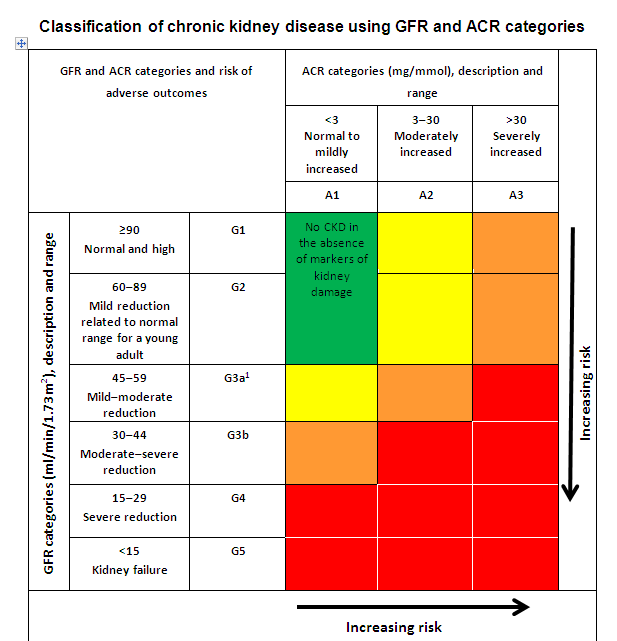
\includegraphics[scale=0.5]{images/gfr-acr-combined-effect.png} & 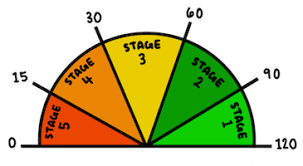
\includegraphics[scale=1.2]{images/gfr1.png} \\
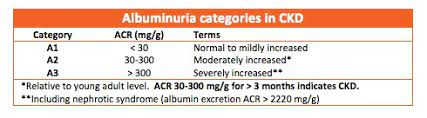
\includegraphics[scale=0.5]{images/acr-stages} & 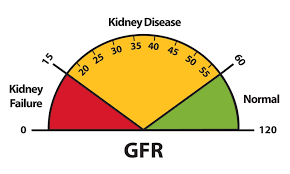
\includegraphics[scale=1.2]{images/gfr2.png} \\
\end{tabular}
\caption{\textbf{GFR, ACR and Kidney Disease (Ref: Google Images)}}
\label{gfr-acr-ckd}
\vspace{0.25cm}
\end{figure}

\flushleft \justifying This study sees how Food Groups affect ACR readings in CKD patients. Moreover, we also wanted to identify what age groups and CKD stages are the most sensitive to food groups. Hence, we studied the effect of Food Groups on ACR for different age groups and CKD stages. Our experiments show no significant relationship between ACR and Food Groups in the population as a whole. We also found that Food Groups show more correlation with ACR for groups with ages under 30 and ACR readings between 3 to 30 than the other groups. In this study, we have utilized Demographics, Dietary Intake, and ACR datasets from NHANES, and CDC. In our study, we have utilized Principle Component Analysis (PCA) to justify the data and find important features in the data. Afterward, we utilized Pearson correlation and regression to study the relation of Food Groups with ACR.

\flushleft \justifying Rest of this report is organized as follows. We will provide a brief literature survey studying the effect of food groups on CKD esp. on ACR and GFR. Additionally, more studies will be mentioned in studies that utilized clustering. Afterward, we will propose our solution and methodology for the study. As part of the solution, we will provide some details about our dataset, data exploration, and dataset generation for our studies. Afterward, we will provide our experimental design. Results and discussion will follow the experimental design. Finally, we will provide conclusion and future work.
\section{Related Work}

\flushleft \justifying In this section, I will provide a literature survey on the association of Food Groups with ACR concerning CKD where data clustering is also utilized. The majority of the research focused on the effect of Nutrients and Drugs on CKD progression. Food group and food subgroup-based study as well as a whole eating pattern-based study is a recent trend. In terms of related work, different categories of related work can be seen to be relevant such as the effects of drugs and nutrients on CKD progression, drugs and nutrients on ACR and GFR, Food Groups/subgroups on CKD progression, Food Groups/subgroups on ACR and GFR, as well as where the above was done by data clustering as well. However, I will primarily focus on studies of Food Groups on ACR. Additionally, I will focus on the usage of clustering in CKD-related studies irrespective if that is for Food Groups or ACR related or not.

\subsection{Food Groups relation with CKD and ACR}
\flushleft \justifying A study ~\cite{Chen2016} studied the relation of plant protein for all-cause CKD mortality. It used statistical models and regression (Cox). It found lower mortality with a high intake of plant protein. Another study ~\cite{Liu2019} used multivariable logistic regression analysis to study vegetarian diets and CKD relations. It found vegetarian diet can be protective. However, one of my past projects as well as other studies ~\cite{Aleix2019} showed that vegetables can also be a risk factor because of high potassium ( and pesticide) content. One research ~\cite{Gutierrez2014} studied five eating patterns and found that processed and fried food are harmful to CKD patients whereas eating patterns with fruits and vegetables are protective. The five eating patterns are convenience (Chinese and Mexican foods, pizza), Plant-based, Sweets/Fats, Southern, and Alcohol/Salads. A study ~\cite{Huang2013} found that the Mediterranean diet has a lower likelihood of having CKD in elderly men. It ~\cite{Huang2013} used unpaired t-test, nonparametric Mann–Whitney test, or chi-square test to Compare CKD and non-CKD men. ~\cite{Ricardo2013} used Cox proportional hazards models with adjustment for covariates and found that healthy lifestyles have a lower risk of all-cause mortality in CKD. A study by Suruya et. al. ~\cite{Tsuruya2015} found that an unbalanced diet is more likely to create adverse clinical outcomes for CKD patients. It used a principal components analysis (PCA) with Promax rotation to derive a smaller set of food groups for analysis. It also used Cox regression with various combinations of covariants. ~\cite{Ricardo2015} found that adherence to a healthy lifestyle decreases risk. ~\cite{Asghari} used multivariable logistic regression and found that high fat and high sugar increase the incidence of CKD. ~\cite{Ahmed2019}.

\subsection{CKD Studies with Data Clustering}
\flushleft \justifying A study on CKD such as ~\cite{Zheng2021} has utilized an unsupervised consensus clustering on 72 baseline characteristics. Depending on patient characteristics clusters were created and clusters/groups of different risks of CKD progression are identified. However, this is not a study on Food Group association with CKD/ACR. ~\cite{LockWood2020} used 11 items on the Kidney Disease Quality of Life symptom profile to identify patient subgroups. This was based on similar observed physical symptom response patterns. However, the goal was to identify subgroups with differing severity. However, this is not a study on Food Group association with CKD/ACR.

\flushleft \justifying Now, I did not see a study utilizing clustering to see how Food Groups are associated with CKD/ACR progression. I also did not come across studies utilizing clustering to find vulnerable groups in terms of sensitivity to food groups for ACR readings. However, a more comprehensive literature survey will be required to conclude this.
\section{Proposed Solution}
In this section, I will provide the steps utilized in my study. Because no significant research is there ~\footnote{I did not come across with some search} on finding relations of food groups with ACR where data clustering is also used, we propose a solution to use data clustering and find associations of food groups with ACR. For data clustering, we propose age and CKD-stage-based studies as well as clustering algorithms such as K-means. Various clustering techniques such as consensus clustering is used for CKD-related studies not for Food groups with ACR studies. Other clustering techniques as well as ensembled clustering techniques can be a future candidate. For the project, we propose age and CKD stage-based study as well as clustering algorithms such as K-means.

\subsection{Methodology Overview}
%\subsection {Approach and Steps}
\flushleft \justifying In the project, I have utilized data from NHANES, CDC. I have taken CDC data on Demographics, Dietary surveys, and Laboratory data ~\cite{CDCDataset}. The data exist from 1996 to 2018. In the project, I have utilized data from 2011 to 2018. I have merged Demographics data, Dietary Intake Data, and ACR readings data from different CDC sources to create the dataset to be utilized in this project. Afterward, I have done data exploration and data curation for data types and missing data. I ensured the output dataset contain data only when data exist for an individual for each aspect such as demographics, diet, and ACR readings. At this point, I have clustered i.e. grouped the data into nine different groups based on Age and ACR readings. Afterward, for each group as well as the total dataset, I find out the most important food groups in the dataset. I have utilized Principle Component Analysis (PCA) to find the important food groups. Afterward, I used Statistical analysis and Pearson correlation to find the correlations of food groups with ACR for each cluster/group. The steps in the proposed solution are given in Figure ~\ref{overall-architecture}.

\tikzstyle{startstop} = [rectangle, rounded corners, minimum width=2cm, minimum height=1cm,text centered, draw=black, fill=red!30]
\tikzstyle{io} = [trapezium, trapezium left angle=70, trapezium right angle=110, minimum width=2cm, minimum height=1cm, text centered, draw=black, fill=blue!30]
\tikzstyle{process} = [rectangle, minimum width=3cm, minimum height=1cm, text centered, draw=black, fill=orange!30]
\tikzstyle{decision} = [diamond, minimum width=3cm, minimum height=1cm, text centered, draw=black, fill=green!30]
\tikzstyle{arrow} = [thick,->,>=stealth]

\subsection{Overall Architecture}
Overall Architecture for  Predict, and Discover Relations of Mortality (and/or ACR) of CKD with Dietary Patterns is given in Figure ~\ref{overall-architecture}.
\begin{figure}[!htb]
\begin{tabular}{c}
\begin{tikzpicture}[node distance=1.5cm]
<TikZ code>
\node (start) [startstop] {Start};
\node (surveydata) [io, text width=8cm, below of=start] {CDC/NHANES Survey data on Demographics, Dietary Intake, and ACR results };
\node (acrdata) [io, text width=2.5cm, below of=surveydata, yshift=-0.25cm, xshift=-3cm] {ACR Data};
\node (fooditems) [io, text width=2cm, right of=acrdata, xshift=5cm] {Food Items};
\node (foodgroups) [io, text width=4cm, below of=fooditems] {Food Group Intake};

\node (proceefoodacr) [process, text width=4cm, below of=acrdata] {Merge ACR, Food Group Intake};
\node (sourcefood) [io, text width=4cm, below of=proceefoodacr] {Source: Food Group Intake Target: ACR};
\node (cluster) [process, text width=5cm, below of=sourcefood] {Clustered Groups based on Age and AC level};
\node (regression) [process, text width=5cm, below of=cluster, yshift=-0.25cm] {Regression/Correlation Relate Food Groups with ACR};
\node (corregression) [io, text width=3cm, below of=regression, xshift=-2cm, yshift = -1cm] {Correlated Food Groups with ACR};
\node (ml) [process, right of=corregression, xshift=3cm] {ML Methods};
\node (acrpredict) [process, text width=5cm, below of=ml] {ACR Predictability};
\node (predicted) [io, text width=3cm, below of=acrpredict, xshift=-2cm] {Predicted ACR from Food Intake};
\node (stop) [startstop, below of=predicted] {Stop};



\draw [arrow] (start) -- (surveydata);
\draw [arrow] (surveydata) -- (acrdata);
\draw [arrow] (surveydata) -- (fooditems);
\draw [arrow] (fooditems) -- (foodgroups);

\draw [arrow] (acrdata) -- (proceefoodacr);
\draw [arrow] (foodgroups) -- (proceefoodacr);

\draw [arrow] (proceefoodacr) -- (sourcefood);
\draw [arrow] (sourcefood) -- (cluster);
\draw [arrow] (cluster) -- (regression);
\draw [arrow] (regression) -- (corregression);
\draw [arrow] (regression) -- (ml);

\draw [arrow] (ml) -- (corregression);
\draw [arrow] (ml) -- (acrpredict);
\draw [arrow] (acrpredict) -- (predicted);
\draw [arrow] (predicted) -- (stop);
\end{tikzpicture}
\end{tabular}
\caption{Overall Methodology: (Clustered) Food Groups Relations with ACR}
\label{overall-architecture}
\end{figure}


\subsection {Dataset}
For the study, I have utilized a dataset from NHANES, CDC. I have taken CDC data on Demographics, Dietary surveys, and Laboratory data ~\cite{CDCDataset}. The data exist from 1996 to 2018. In the project, I have utilized data from 2011 to 2018. I have used a semi-automated method to convert the data from CDC to be utilized in this project.


\subsubsection{Data Synthesis}
\noindent Initially, all the Demographics data from 2011 to 2018 are merged into one big demographic data.
Then all ACR reading data from 2011 to 2018 were merged into one big dataset for ACR readings. ACR data have the participant id in it. Afterward, all dietary intake data from 2011 to 2018; also for multiple days of intake data are merged into one large dietary intake data. At this point, these demographics, ACR, and Dietary intake data were mapped, and only matching data were merged into one big dataset having demographics, ACR, and dietary intake data. To create clusters, then, I divided them into 9 different clusters. The clusters used age groups such as 0 to 30, 31 to 60, and over 61. For each age group, I further divided the data using ACR readings such as less than 3, 3 to 30, and over 30. This created 9 clusters in addition to the data having all data together. Figure ~\ref{clusters-table} provides the details of the clusters. ACR values are used as the target variable for the analysis. I used PCA to find out important food groups while I used statistical analysis and Pearson correlation to find potential associations with Food groups and ACR.


\begin{figure}
\begin{tabular}{|p{4cm}|p{6cm}|p{6cm}|}
\hline
\textbf{Class} & \textbf{Age} & \textbf{ACR}\\
\hline
0 & all & all \\
\hline
1 & 0 to 30 & $<$ 3 \\
\hline
2 & 0 to 30 & 3 to 30 \\
\hline
3 & 0 to 30 & Over 30 \\
\hline
4 & 31 to 60 & $<$ 3 \\
\hline
5 & 31 to 60 & 3 to 30 \\
\hline
6 & 31 to 60 & Over 30 \\
\hline
7 & Over 60 & $<$ 3 \\
\hline
8 & Over 60 & 3 to 30\\
\hline
9 & Over 60 & Over 30\\
\hline

\end{tabular}
\caption{\textbf{All the Clusters/Groups of Data}}
\label{clusters-table}
\vspace{0.25cm}
\end{figure}

\flushleft \justifying While I primarily utilized Age and ACR-Induced CKD stages for data clustering, however, I also want to propose clustering algorithms such as K-Means and K-Medians. Other clustering methods as well as Consensus/Ensembled clustering algorithms will also be a future candidates. K-means can be a starting point. I have provided a K-Means algorithm for data clustering. Several features such as Age, ACR, GFR, Blood Pressure, or similar critical CKD data can be used to center the data around to create clusters. The K-means algorithm is provided in Algorithm ~\ref{k-means-algorithm}.

\subsubsection{K-Means Clustering}
\renewcommand{\labelitemi}{$$}

\begin{algorithm}
\caption{Cluster Data using K-Means}
\label{k-means-algorithm}
\begin{algorithmic}
\STATE \textbf{Goal: Cluster the Data according to K-Means algorithm}\vspace{0.10cm}
\STATE Let k = 10
\STATE Find k random tuples to act as the initial data/cluster centers
\vspace{0.10cm}

\WHILE {further data can be moved from cluster to cluster or 5000 times}
\STATE Take (Age, ACR, GFR, Blood Pressure) as the primary metrics to center the data around
\STATE Centre all the data around the 10 centers (Age, ACR, GFR, and Blood Pressure)
\STATE Find the new mean for these clusters
\STATE Again center around (Age, ACR, GFR, Blood Pressure)

\ENDWHILE

\vspace{0.10cm}
\end{algorithmic}
\end{algorithm}


\flushleft \justifying I have implemented a proof of KMeans clustering to cluster the data into 10 clusters. Cluster count and the features for the clusters can easily be custom configured. Figure ~\ref{kmeans-python} shows the code for the proof of concept implementation. Figure ~\ref{cluster-plot} shows the clusters in an image. The GitHub repository will have the complete code, also the output from the code. Now, the analysis can be done with these clusters as well in addition to the clusters I created before.

\begin{figure}
\begin{tabular}{c}
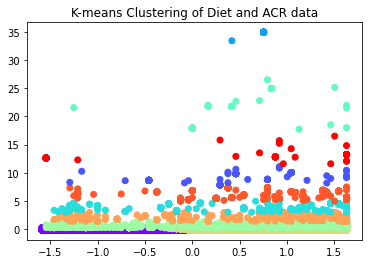
\includegraphics[scale=0.6]{images/kmeans/cluster-plot.png} \\
\end{tabular}
\caption{\textbf{10 Clusters created with KMeans Algorithm}}
\label{cluster-plot}
\vspace{0.25cm}
\end{figure}

\begin{figure}
\begin{tabular}{c}
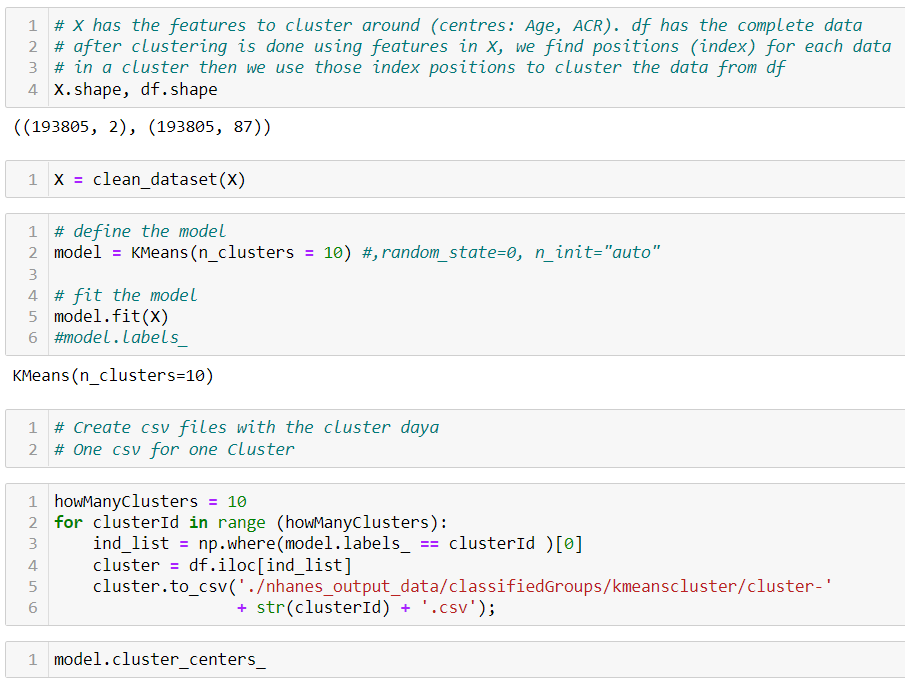
\includegraphics[scale=0.6]{images/kmeans/kmeans-clustering-implementations.png} \\
\end{tabular}
\caption{\textbf{KMeans Code for Clustering }}
\label{kmeans-python}
\vspace{0.25cm}
\end{figure}
\section{Experiments}
I used the Experiments as shown in Figure ~\ref{experiment-regular-clustering} to find associations between dietary patterns (i.e. Food Groups) and ACR. For the regression experiments, both Actual Values and Normalized values are used. However, I have reported only regression-based results based on the experiments done on normalized data. Similar experiments could be done with the clusters that I created using K-Means. I have provided experiment design for K-Means Clustered Data in Figure ~\ref{experiment-regular-kmeans-clustering} to conduct similar experiments. These experiments on Clustered Data could discover additional valuable relations and associations.

\begin{figure}[!htb]
%\begin{table}[!htb]
\caption{\textbf{Effect of Food Groups on ACR} \\ use Age and ACR based clustering}
\label{experiment-1}
\vspace{0.25cm}
\begin{tabular}{| p{4cm} | p {12cm} | }
\hline
\noindent \textbf{Primary Input Dataset:} & Clustered dataset with demographics, and dietary intake data from 2011 to 2018. Dietary intake amounts for food groups.\\
\hline
\noindent \textbf{Target Variable:} & Albumin to Creatinine Ratio (ACR) \\
\hline
\noindent \textbf{Experiment 1.1:} & { Identify contributing and important food groups in the input dataset using PCA for the cluster. } \\
\hline
\noindent \textbf{Experiment 1.2:} & { Find out correlation (using Pearson’s correlation, between ACR Values and important food groups as found using PCA in experiment 1.1.} \\
\hline
\noindent \textbf{Experiment 1.3:} & { Find out regression coefficients of the important food groups (PCA) with ACR using various Regression techniques such as Linear and Polynomial Regression, Linear and Polynomial Regression with Cross Validations, Bayesian and Random Forest Regression with or without Cross Validations} \\
\hline
\end{tabular}
\label{experiment-regular-clustering}
%\end{table}
\end{figure}

\begin{figure}[!htb]
%\begin{table}[!htb]
\caption{\textbf{Effect of Food Groups on ACR} \\ use \textbf{K-Means Clustering}}
\label{experiment-1}
\vspace{0.25cm}
\begin{tabular}{| p{4cm} | p {12cm} | }
\hline
\noindent \textbf{Primary Input Dataset:} & K-Means Clustered dataset with demographics, and dietary intake data from 2011 to 2018. Dietary intake amounts for food groups.\\
\hline
\noindent \textbf{Target Variable:} & Albumin to Creatinine Ratio (ACR) \\
\hline
\noindent \textbf{Experiment 2.1:} & { Identify contributing and important food groups in the input dataset using PCA for the K-Means Clustered data. } \\
\hline
\noindent \textbf{Experiment 2.2:} & { Find out correlation (using Pearson’s correlation, between ACR Values and important food groups as found using PCA in experiment 1.1.} \\
\hline
\noindent \textbf{Experiment 2.3:} & { Find out regression coefficients of the important food groups (PCA) with ACR using various Regression techniques such as Linear and Polynomial Regression, Linear and Polynomial Regression with Cross Validations, Bayesian and Random Forest Regression with or without Cross Validations. Use K-Means Clustered dataset} \\
\hline
\end{tabular}
\label{experiment-regular-kmeans-clustering}
%\end{table}
\end{figure}

\pagebreak

\section {Results and Discussion}
In this section, I will provide and discuss the results of the project. I will also provide limitations and challenges.

\subsection{Finding Important Food Groups}
\flushleft \justifying I have utilized PCA to find out the important food groups in the clusters. PCA finds the importance of the food groups in the dataset for all the clusters. PCA variance and PCA Component Configurations for the cluster Age $>$ 60, and ACR $<$ 3 are given in Figure ~\ref{pca-v-food-comp}. Contributing Food Groups in the data are provided in Figure ~\ref{cluster-food-contribution}. From Figure ~\ref{pca-v-food-comp}, we see that the most important food groups for the Class: age $>$ 60, ACR $>$ 3, ACR $<$ 30 for the 1st PCA component are Total Fat, Monounsaturated Fatty Acids; Important food groups for the second PCA component are Carbohydrate, Sugar, Cholesterol (-), and Protein. 3rd PCA component shows Fibre, Sugar (-), Cholesterol (-) are important where 4th PCA component shows Protein, Total Poly Fat (-) are important. In most cases, I considered upto three or four PCA components because that can describe around 90\% of the data. From the experiment, I see that the important food groups for different clusters are very consistent with each other. It may mean that food groups taken by the population in the clusters are closely matched.

\begin{figure}
\begin{tabular}{c}
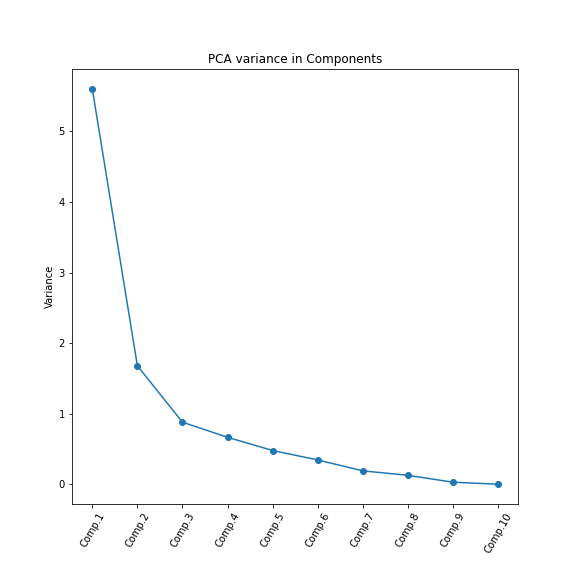
\includegraphics[scale=0.4]{images/pca_components_variance} \\
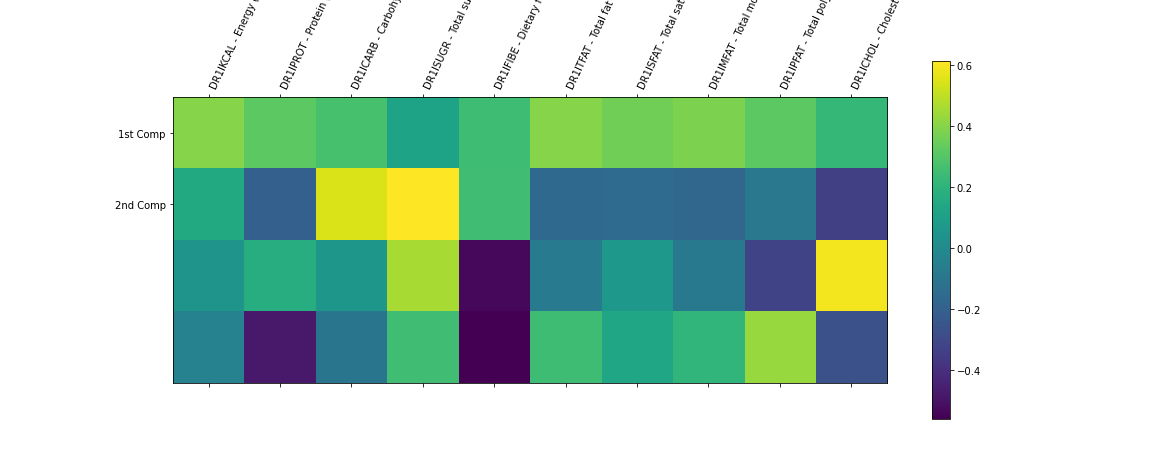
\includegraphics[scale=0.4]{images/pca_food_groups_what_contributes_to_PCA_components.png} \\
\end{tabular}
\caption{\textbf{PCA variance (top) and PCA Component Configurations for the cluster Age $>$ 60, and ACR $<$ 3 (bottom) }}
\label{pca-v-food-comp}
\vspace{0.25cm}
\end{figure}

\begin{figure}
\begin{tabular}{c}
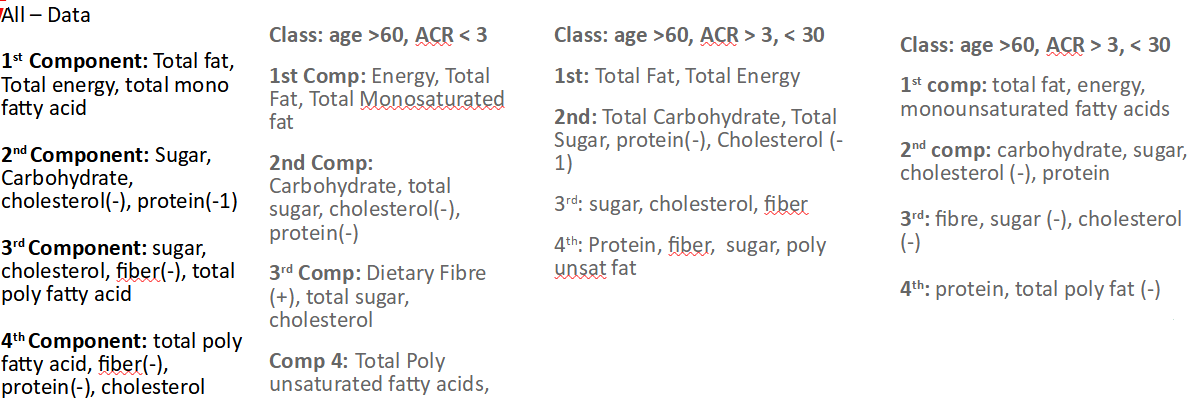
\includegraphics[scale=1]{images/important-features-food-groups.png} \\
\end{tabular}
\caption{\textbf{Contributing Food Groups in the Data Clusters}}
\label{cluster-food-contribution}
\vspace{0.25cm}
\end{figure}

\subsection{Food Group ACR Association}
Correlations between Food Groups and ACR are given in Figure ~\ref{corr-acr-food}. It also shows the correlation based on groups created on Age and ACR CKD stages. I have utilized Pearson correlation on the data after PCA. For example, Figure ~\ref{corr-acr-food} shows
that for Class 2 [Age (0, 30) ACR (3, 30)], Protein, and Fat have a correlation of -0.041 with ACR, Carbohydrate has a correlation of -0.038, and Poly unsaturated has -0.036 where Mono unsaturated has a correlation of -0.032 with ACR. For the Class 5 [Age (30, 60), ACR (3, 30)], Protein correlates -0.011, and Monounsaturated Fat correlates -0.011.


\begin{figure}
\begin{tabular}{cc}
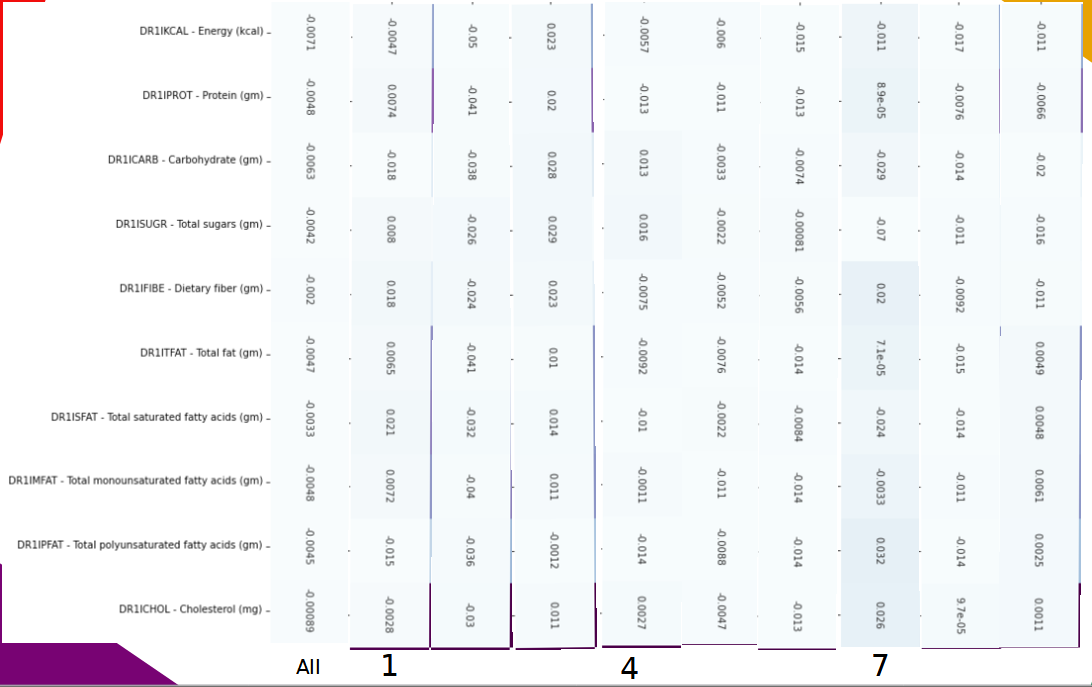
\includegraphics[scale=0.7]{images/groups-and-foods-and-correlations} \\
\end{tabular}
\caption{\textbf{Correlation of Food Groups with ACR by Age and CKD stage groups}}
\label{corr-acr-food}
\vspace{0.25cm}
\end{figure}


\begin{figure}
\begin{tabular}{c}
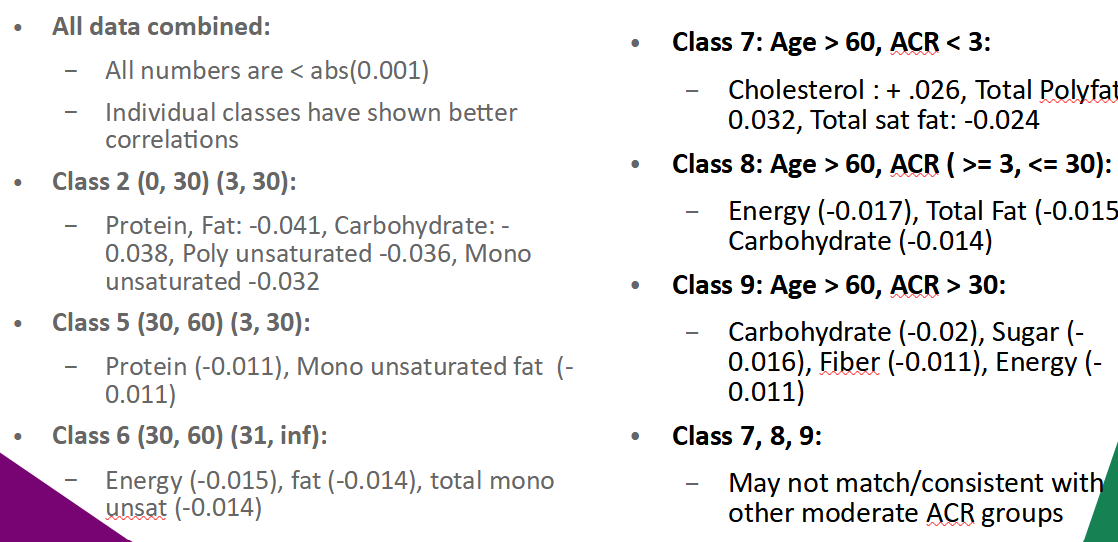
\includegraphics[scale=0.7]{images/noticeable-corr-and-food-groups.png} \\
\end{tabular}
\caption{\textbf{Some Higher Correlation numbers of Food Groups with ACR by Age and CKD stage groups}}
\label{corr-acr-food22}
\vspace{0.25cm}
\end{figure}

\subsection{Regression Coefficients}
\flushleft \justifying In this analysis, I applied regressions to find the regression coefficients i.e. to what extent a particular variable (such as the food groups) is affecting ACR. I have applied several approaches such as Linear Regression, Linear Regression with 10-Fold Cross Validation, Polynomial Regress with or without K-Fold Cross Validation, Bayesian and Random Forest regressor with or without polynomial data, and K-fold cross-validation. First, I will provide the coefficients that I found. Afterward, I will explain the significance of the coefficients. Figure ~\ref{clusters-table} provides the details of the clusters. Figure ~\ref{food-groups-abbr} shows the full form of the abbreviated food groups used in Figure ~\ref{reg-coef-food-acr}.

\flushleft \justifying Figure ~\ref{reg-coef-food-acr} shows that For Class 2 [Age(0 to 30), ACR (3 to 30) ] Higher Energy (Calorie) intake can lead to increased ACR readings. All Forms of Regression show the same. Afterward, all regression types show that Poly Unsaturated Fatty Acids have the 2nd highest contribution to ACR for Group 2. Then, all regression types show that Cholesterol has the 3rd highest contribution to ACR for Group 2. Mono Unsaturated Fatty Acids have the next level of effectiveness. Results from Linear Regression vary slightly from the other regressions I used. The code output kept at $codeoutput/regression-foodgroup-and-acr.pdf$ shows that R2 values are not significant. However, PCA data shows that Food Groups represent the data well. These may need further attention. The code $code/regression-foodgroup-and-acr.ipynb$ can be executed for any other class/cluster to find the relation of Food Groups for that Cluster. Also, the code can be applied to the Clusters created with KMeans to find relations of Food Groups with ACR. This may also show the most vulnerable groups/clusters and food groups.


\begin{figure}
\begin{tabular}{|p{4cm}|p{12cm}|}
\hline
Food Groups & Ener, Pro, Carbo, Sug, Fib, Fat, SatFatAcid, MonoUnsatFatAcid, PolyUnSatFatAcid, Choles \\
\hline
Class 2, LinearRegressionNormalizedValues & [-0.48, 0.05, 0.24, -0.15, -0.03, -0.34, 0.37, 0.17, 0.19, -0.09] \\
\hline
\hline
Class 2, LinearRegressionCrossValidation & [-0.36, -0.22, -0.05, -0.02, -0.01, -0.06, -0.01, -0.22, -0.31, -0.29] \\
\hline
Class 2, PolynomialRegressionCrossValidation & [-0.36, -0.22, -0.05, -0.02, -0.01, -0.07, -0.01, -0.23, -0.66, -0.29] \\
\hline
Class 2, BayesianPolynomialCrossValidation & [-0.36, -0.22, -0.05, -0.02, -0.01, -0.06, -0.01, -0.22, -0.31, -0.29] \\
\hline
Class 2, RandomForestRegressorCrossValidation & [-0.35, -0.21, -0.05, -0.02, -0.01, -0.06, -0.01, -0.22, -0.3, -0.28] \\
\hline
\end{tabular}
\caption{\textbf{Regression Co-Efficients of Food Groups with ACR}}
\label{reg-coef-food-acr}
\vspace{0.25cm}
\end{figure}

\begin{footnotesize}
\begin{figure}
\begin{tabular}{|p{4cm}|p{6cm}|}
\hline
Ener & Energy \\
\hline
Pro & Protein \\
Carbo & Carbohydrate \\
\hline
Sug & Sugars \\
\hline
Fib & Fiber \\
\hline
Fat & Fat \\
\hline
SatFatAcid & Saturated Fatty Acids \\
\hline
MonoUnsatFatAcid & Mono Unsaturated Fatty Acids \\
\hline
PolyUnSatFatAcid & Poly Unsaturated Fatty Acids \\
\hline
Choles & Cholesterol \\
\hline

\end{tabular}
\caption{\textbf{Food Groups: Short and Long Names}}
\label{food-groups-abbr}
\vspace{0.25cm}
\end{figure}

\end{footnotesize}

\subsection {Limitations}
\flushleft \justifying In the study, I have used the food groups found in the Dietary Intake survey. Instead, Food Groups and Sub-Groups from USDA could be used to align with USDA and other studies utilizing USDA food groups. I faced several challenges on this such as I found only 2015-2016 USDA food group data. It did not seem sufficient to assign food groups and sub-groups to the entire dataset I created. Hence, the further discovery of Data on USDA food groups will be required. I have utilized Age and ACR-Induced CKD stages for data clustering. The age group is taken from one of several approaches used for medical studies. However, a clustering algorithm such as K-Means could add value. Several CKD studies not specific to ACR utilized clustering such as Consensus/Ensembled Clustering. This study could benefit from such clustering. Additionally, I have utilized ACR as the target based on data availability. A measure such as GFR is prominently used in CKD stage determination. Hence, GFR is a better candidate than ACR to be used as the target variable. Ideally, a combination of GFR and ACR gives the true picture of CKD condition. Hence, combined ACR/GFR metric as the target variable will bring more values to the association outcome/result. Also, mortality and survival could be target variables as the first step or as the 2nd step target variable. If 2nd step ACR/GFR association can be used as the input.

\flushleft \justifying I have implemented K-Means clustering of the dataset to create 10 clusters. The cluster data can be found on GitHub under $cas-764-food-group-acr-cluster/ code/ nhanes\_output\_data \\ /classifiedGroups/ kmeanscluster$. The analysis that I have done with the initial clustered data, the same can be done with the K-Means clustered data. I could do PCA Analysis, Pearson Correlation, and all the regressions that I did (Bayesian, RandomForst, Regression with Cross Validation). Further, I could change the features to center the cluster around. These analyses could further bring clarity to the association between Food groups and ACR, and subsequently to Mortality and Survival.

\flushleft \justifying  Also, an extensive data exploration could be done at the beginning to see how the data fits into the study. A study could be R Square analysis. In my regression analysis, R Square is used; however, it could be done on a large scale at the start and then data adjustment leading to a significant R square number for the entire dataset and the clusters could make the study more valuable. Also, a pair-wise correlation study could filter out correlated features and food groups.

\section{Applications}
\flushleft \justifying The approach taken in this study can be utilized in a generic way where we want to find relations associations of some input variables to a target variable. For example, I have studied the association of Food Groups with ACR. With relevant datasets, the association of Food Groups with ACR/GFR can be discovered as well. Additionally, the regression coefficients that I am trying to find out, the same approach can be utilized in many fields such as finance, and surveillance. For example, in a target tracking application in a cluttered environment, the environmental features, as well as performance metrics, can be studied to find out how these affect the accuracy. Based, on this the algorithm could dynamically adapt to make the target tracking more accurate.



\section{Conclusion}

\flushleft \justifying %Chronic Kidney Disease (CKD) is highly prevalent today. CKD can lead to kidney failure and death. CKD has no permanent cure. Hence, the treatment options involve drugs, lifestyle, and food choices. The majority of the research studied the effects of Drugs and nutrients on CKD progression. The effect of food and eating patterns on CKD has attracted recent attention. However, the research is not significant yet. Hence,
\flushleft \justifying In this study, I have studied the effect of food groups on a CKD diagnostic marker called Urine Albumin Creatinine Ratio (ACR). Urine ACR can determine the severity of CKD. This study finds out how Food Groups affect ACR readings and also the severity in CKD patients. Moreover, we also identified age groups and CKD stages that are the most sensitive to food groups. We have utilized Age and ACR reading-based Clusters and also explored on K-Means clustering. In this study, we have utilized Demographics, Dietary Intake, and ACR datasets from NHANES, and CDC. In this study, I have utilized Principle Component Analysis (PCA) to justify the data and find the important features such as Food Groups in the data. Afterward, I utilized Pearson correlation and regression to study the relation of Food Groups with ACR. My experiments show no significant relationship between Food Groups and ACR in the total population. I also found that Food Groups show more correlation with ACR for groups with ages under 30 and ACR readings between 3 to 30. I also have applied several regression techniques such as Linear and Polynomial Regression, Linear and Polynomial Regression with Cross Validations, and Bayesian and Random Forest Regression with or without Cross Validations to find out the regression coefficients of the food groups affecting ACR. Experiments show that Higher Energy (Calorie) intake can lead to increased ACR readings. All Regression techniques show the same for calories. Afterward, all regression techniques showed that Poly Unsaturated Fatty Acids have the 2nd highest contribution to ACR for Cluster 2. All regression techniques also showed that Cholesterol has the 3rd highest contribution to ACR for Cluster 2.

\subsection{Future Work}
\flushleft \justifying Several immediate future extensions of this study can include integrating data from 1996, utilizing USDA food groups, conducting experiments on the KMeans clustered data that I generated, or utilize Consensus Clustering to cluster data, and using Machine Learning to predict ACR from dietary intake.

\flushleft \justifying The research focus can also include finding groups that are the most sensitive to food groups for ACR and GFR. Studies can place the combined effect on ACR/GFR as the target variable to find relations with food groups and sub-groups. I did not come across studies that study food groups' effect on the combined GFR and ACR metrics. Additional studies can focus on how food groups' effect on ACR/GFR propagates to Mortality and Survival of CKD patients. Survival and Mortality can use food groups and sub-groups as the input variables or can use the effect on ACR/GFR metrics as the input.
%\section{References}

\begin{thebibliography}{1}

\bibitem{Olga2022}  Latent Class Cluster Analysis: Selecting the number of clusters
https://www.sciencedirect.com/science/article/pii/S2215016122001273

\bibitem{CDCDataset}Dietary Patterns of Patients with Chronic Kidney Disease: The Influence of Treatment Modality
https://www.ncbi.nlm.nih.gov/pmc/articles/PMC6723967/

\bibitem{Zheng2021} Subtyping CKD Patients by Consensus Clustering: The Chronic Renal Insufficiency Cohort (CRIC) Study: https://jasn-asnjournals-org.libaccess.lib.mcmaster.ca/content/32/3/639

\bibitem{LockWood2020} Physical Symptom Cluster Subgroups in Chronic Kidney Disease
https://www.ncbi.nlm.nih.gov/pmc/articles/PMC7353908/

\bibitem{USRDS2022} United States Renal Data System. https://www.niddk.nih.gov/about-niddk/strategic-plans-reports/usrds . This site will have agw group based CKD studies and reports.


\bibitem{Chen2016}  	Chen X, Wei G, Jalili T, Metos J, Giri A, Cho ME, Boucher R, Greene T, Beddhu S: The associations of plant protein intake with all-cause mortality in CKD. Am J Kidney Dis 67: 423–430, 2016 (26)

\bibitem{Liu2019} [26]	Liu, Hao-Wen; Tsai, Wen-Hsin; Liu, Jia-Sin; Kuo, Ko-Lin. 2019. "Association of Vegetarian Diet with Chronic Kidney Disease." Nutrients 11, no. 2: 279.

\bibitem{Aleix2019} Aleix Cases, Secundino Cigarran-Guldris, Sebastian Mas, and Emilio Gonzalez-Parr. Vegetable-Based Diets for Chronic Kidney Disease? It Is Time to Reconsider. Nutrients. 2019 Jun; 11(6): 1263.

\bibitem{Gutierrez2014} Gutierrez O.M., Muntner P, Rizk D.V., McClellan W.M., Warnock D.G., Newby P.K., Judd S.E.: Dietary patterns and risk of death and progression to ESRD in individuals with CKD: A cohort study. Am J Kidney Dis 64: 204–213, 2014  (27)

\bibitem{Huang2013} Huang X., Jime nez-Moleo J. J., Lindholm B., Cederholm T., Arnoldv J., Rise rus U., Sjogren P., Carrero J. J.: Mediterranean diet, kidney function, and mortality in men with CKD. Clin J Am Soc Nephrol 8: 1548–1555, 2013 (28)

\bibitem{Ricardo2013} Ricardo A. C., Madero M., Yang W., Anderson C., Menezes M., Fischer M.J., Turyk M., Daviglus M.L., Lash J.P.: Adherence to a healthy lifestyle and all-cause mortality in CKD. Clin J Am Soc Nephrol 8: 602–609, 2013 (30)

\bibitem{Tsuruya2015} Tsuruya K., Fukuma S., Wakita T., Ninomiya T., Nagata M., Yoshida H., Fujimi S., Kiyohara Y., Kitazono T., Uchida K., Shirota T., Akizawa T., Akiba T., Saito A., Fukuhara S.: Dietary patterns and clinical outcomes in hemodialysis patients in Japan: A cohort study. PLoS One 10: e0116677, 2015 (31)

\bibitem{Ricardo2015} Ricardo A.C., Anderson C.A., Yang W., Zhang X., Fischer M. J., Dember L. M., Fink J. C., Frydrych A., Jensvold N. G., Lustigova E., Nessel L. C., Porter A. C., Rahman M., Wright Nunes J. A., Daviglus M. L., Lash J. P.;  CRIC Study Investigators: Healthy lifestyle and risk of kidney disease progression, atherosclerotic events, and death in CKD: Findings from the Chronic Renal Insufficiency Cohort (CRIC) Study. Am J Kidney Dis 65: 412–424, 2015 (17)

\bibitem{Asghari} Golaleh Asghari, Mehrnaz Momenan, Emad Yuzbashian, Parvin MirmiranEmail author and Fereidoun Azizi. Dietary pattern and incidence of chronic kidney disease among adults: a population-based study

\bibitem{CDCDataset} CDC data on: Demographics, Dietary Survey, Examination, Laboratory, Questions. https://wwwn.cdc.gov/nchs/nhanes/Search/DataPage.aspx?Component=Dietary


\bibitem{Ahmed2019} Sayed Ahmed, Youcef Derbal: Effect of Dietary Patterns on CKD Mortality, and Impact of Dietary Recommendations Shift on Chronic Kidney Disease: $https://www.researchgate.net/publication/337544477\_Effect\_of \_Dietary\_Patterns\_on \_CKD\_Mortality \_and \_Impact\_of\_Dietary
\_Recommendations \_Shift\_on\_Chronic\_Kidney \_Disease$








\end{thebibliography}
\pagebreak
\section{Appendix}

\subsection{Code}
I have placed the code used for the project at: https://github.com/sayedmcmaster/cas-764-food-group-acr-cluster/code %\footnote{My understanding is this subsection ideally belongs to appendix}. https://github.com/sayedmcmaster/cas-764-food-group-acr-cluster/codeoutput A list of the files and purpose is given below:

%\begin{figure}
%\begin{tabular}{|c|c|}
%\hline
%File & Purpose\\
%\hline
%$xpt\_to\_csv\_all\_files\_in\_a\_folder.ipynb$ & converts SAS XPT data files to CSV files. It converts demographics, ACR Lab Data, and Dietary Intake data into CSV files. It shows a drop-down to select the Input File and the Input data format file and then convert it. It could convert any other XPT data file such as Blood Pressure data files to CSV files as well. \\
%\hline
%\end{tabular}
%\caption{\textbf{GFR, ACR and Kidney Disease (Ref: Google Images)}}
%\label{gfr-acr-ckd-methodology}
%\vspace{0.25cm}
%\end{figure}


\subsection{Dataset Generation}
Initially, I wrote and used Python code ($xpt\_to\_csv\_all\_files\_in\_a\_folder.ipynb$) to generate data files for each year (Demographics, ACR, Dietary Intake). Then I brought the data into MS SQL Server. Then wrote and used Stored Procedures to combine each category of data, and then used another stored procedure (dietaryIntakeDataForClassificationAndAnalysis. StoredProcedure. sql) to join all these data to create the big dataset for analysis. The stored procedures can be found on GitHub under 'sayedmcmaster/cas-764-food-group-acr-cluster/code/SQL/storedprocedures/' and in Figure ~\ref{sp-combine}. This is what I used initially. However, later I wrote another Python code $automated\_xpt\_to\_csv\_all\_files.ipynb$ that can create CSV files from XPT one by one iteratively. This code ideally can combine all data input given in one shot provided the columns align. Also, wrote another Python code to merge one category of data files (I also have a stored procedure). Both approaches have some pros and cons. I am using and planning to use them as they seem appropriate. \footnote{Because the code and SQLs are only for my use, I am not making them perfect considering coding standards and performance}

\begin{figure}[!htb]
\begin{tabular}{c}
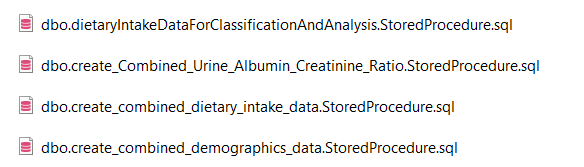
\includegraphics[scale=1]{images/datasetgenerationcode/create-data-set.png} \\
\end{tabular}
\caption{\textbf{Stored Procedures to Combine Data and to create big dataset}}
\label{sp-combine}
\vspace{0.25cm}
\end{figure}

\subsubsection{Code for Automated (semi-automated) CSV Data generation from XPT files}
File: $automated\_xpt\_to\_csv\_all\_files.ipynb$, Figure: ~\ref{automated-data-year}, ~\ref{automated-data-traverse}, ~\ref{automated-data-csv}

\begin{figure}[!htb]
\begin{tabular}{c}
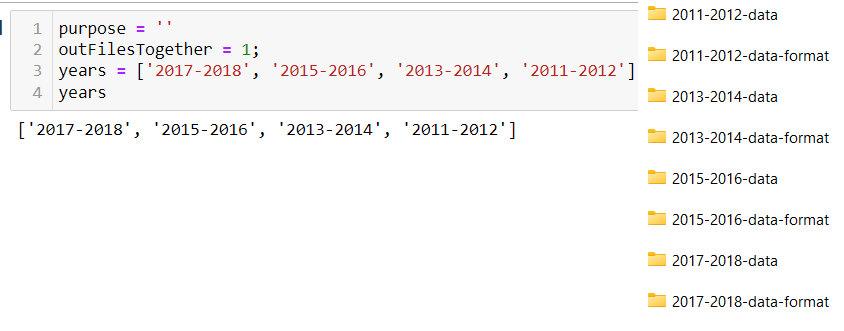
\includegraphics[scale=1]{images/datasetgenerationcode/set-years.png} \\
\end{tabular}
\caption{\textbf{Set all years to work on, Data Folder Structure}}
\label{automated-data-year}
\vspace{0.25cm}
\end{figure}

\begin{figure}[!htb]
\begin{tabular}{c}
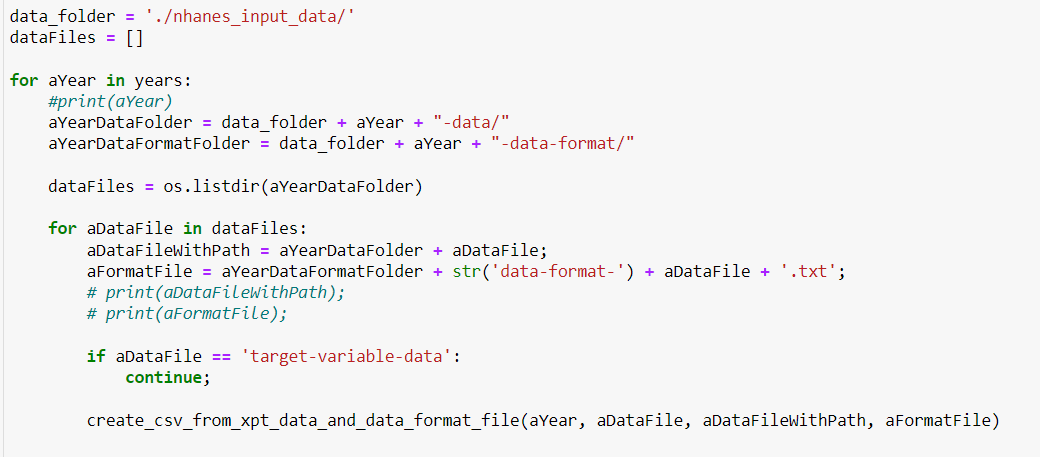
\includegraphics[scale=0.8]{images/datasetgenerationcode/convert-all-input-datafiles-for-multiple-years-into-csv-files.png} \\
\end{tabular}
\caption{\textbf{Traverse all data files and send them for conversion to CSV files}}
\label{automated-data-traverse}
\vspace{0.25cm}
\end{figure}


\begin{figure}[!htb]
\begin{tabular}{c}
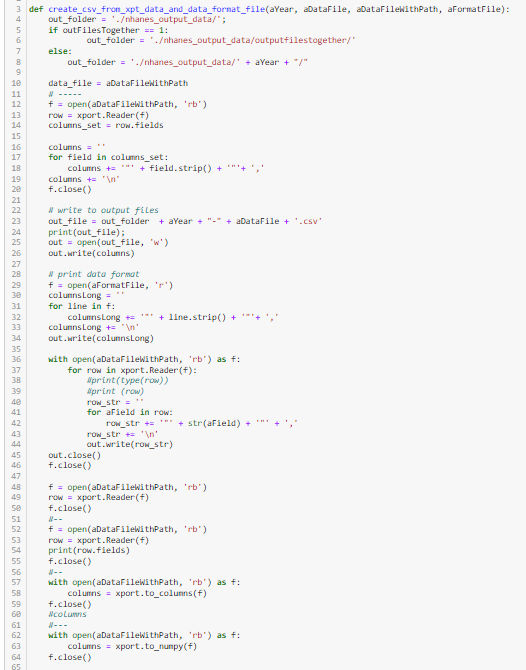
\includegraphics[scale=1]{images/datasetgenerationcode/code-writing-data-one-file-at-a-time.png} \\
\end{tabular}
\caption{\textbf{Code for Automated (semi-automated) Dataset Generation. create the CSV files with data}}
\label{automated-data-csv}
\vspace{0.25cm}
\end{figure}

%\pagebreak
\subsubsection{Merge Data Files from Multiple Years }
File: $merge-multiple-csv-files-with-python$, Figure: ~\ref{merge-data-files}, Purpose: We can configure this file to merge all demographics data or all dietary data, or all ACR data from multiple years into one. Some column alignments are needed in some cases where columns differ from year to year. I used Winmerge software to see the differences in data format.
\begin{figure}[!htb]
\begin{tabular}{c}
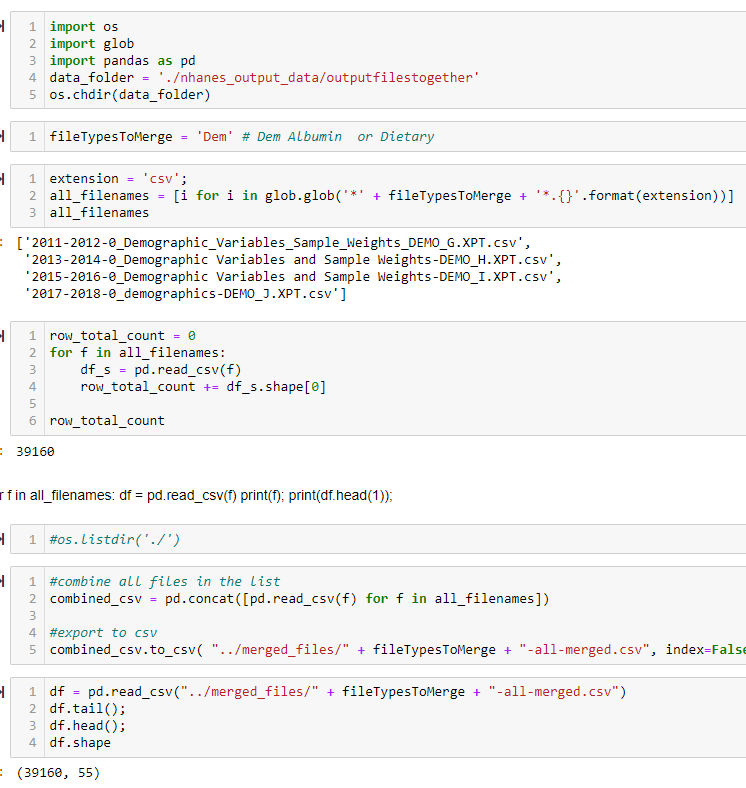
\includegraphics[scale=1]{images/datasetgenerationcode/merge-demographics-files.png} \\
\end{tabular}
\caption{\textbf{Merge Data Files from Multiple Years by category}}
\label{merge-data-files}
\vspace{0.25cm}
\end{figure}

%\pagebreak
\subsubsection {Cluster/Group Generation}
I have written a code in Python to create clusters as can be seen in Figure ~\ref{python-cluster}.
File: $cleaned-classifyDataBasedOnAgeAcrLevelAndThenTakeTheDietaryIntakeData.ipynb$ can be found on GitHub under the code folder. I also have written and used stored procedures to create clusters such as
$dbo.create\_a\_class\_group\_dataset.StoredProcedure.sql$ and $dbo.create\_classified\_dataset.StoredProcedure.sql$. These can be found in GitHub under code/SQL/storedprocedures/. I have used both Python and Stored Procedures to create clusters and verify that the output is correct \footnote{If data types in database tables are not correct for age, ACR then Python may not give correct clusters. Python code needs to use type casting}.

\begin{figure}[!htb]
\begin{tabular}{c}
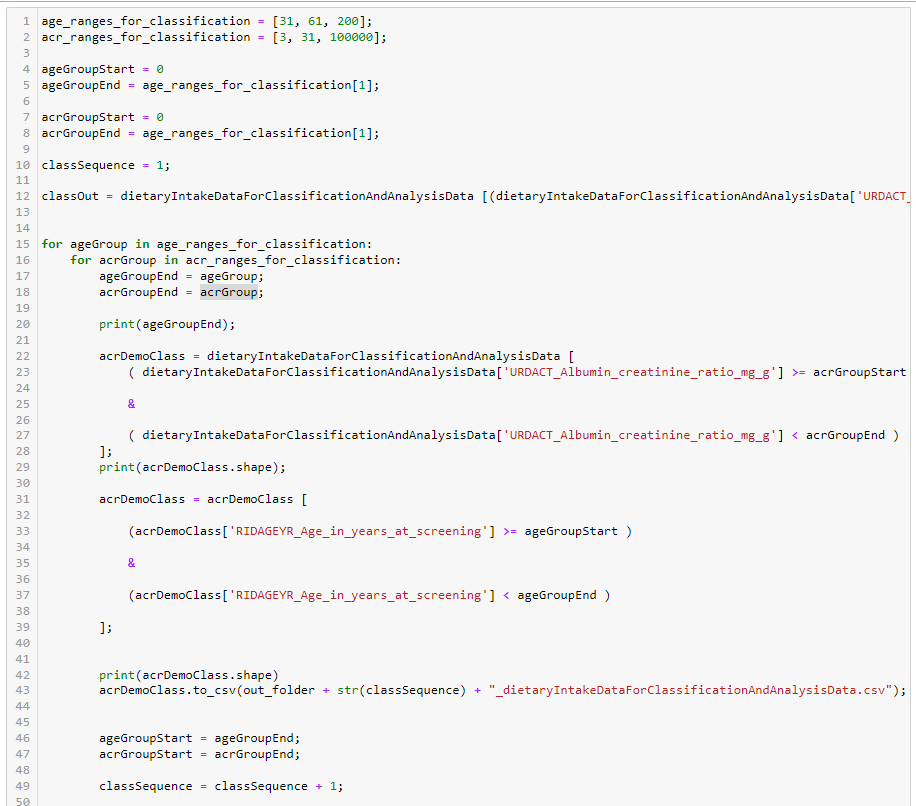
\includegraphics[scale=0.8]{images/datasetgenerationcode/cluster-python-code.png} \\
\end{tabular}
\caption{\textbf{Python Code to Create Clusters}}
\label{python-cluster}
\vspace{0.25cm}
\end{figure}


\subsection{Correlation of Food Groups with ACR}
Code File: $cleaned-foodgroup-acr-ratio-relation-by-agegroups-and-foods$. The code file can be found on GitHub under 'sayedmcmaster/cas-764-food-group-acr-cluster/tree/main/code/Exploratory Analysis/'. This code file generated the important food groups and correlation results as shown under the Results and Discussion section in figures ~\ref{pca-v-food-comp}, ~\ref{cluster-food-contribution}, ~\ref{corr-acr-food}, and ~\ref{corr-acr-food22}.

\subsection{Regression Coefficients contributing to ACR readings}
Code File: $regression-foodgroup-and-acr.ipynb$. The code file can be found on GitHub under: 'sayedmcmaster/cas-764-food-group-acr-cluster/tree/main/code'. This code file uses approaches such as Regression, Polynomial Regression, Random Forest, and Bayesian to find correlation coefficients of the food groups contributing to ACR readings. It finds correlations for the entire dataset as well as for the groups.

\subsection{K-Means Clustering}
I have implemented a proof of concept K-means algorithm to cluster the data. The data is clustered based on Age and ACR levels. However, if other data such as blood pressure is brought from NHANES, CDC then the clustering can also be updated with Age, ACR, and Blood Pressure. It just will need an update to the list of features to center around.
Code File: $kmeans-cleaned-and-code-combined-in-less-number-of-blocks$. The cluster data created with Kmeans can be found under $code/nhane_output_data/classifiedGroups/kmeanscluster$.

\end{document}